\levelstay{The Four Fourier Transforms}

There are four different types of Fourier transform, corresponding
to the four different ways in which data may be sampled in time: data
may be known at discrete or continuous times, and over a finite or
infinite extent of time. The four transforms are 
\begin{itemize}
  \item Fourier transform (FT) - continuous time, infinite extent 
  \item Fourier series (FS) - continuous time, finite extent 
  \item Discrete time Fourier transform (DTFT) - discrete time, infinite extent 
  \item Discrete Fourier transform (DFT) - discrete time, finite extent 
\end{itemize}
Each of these transforms is useful in making calculations and in developing theoretical understanding, but in the lab where we have discretely sampled or generated data over finite durations of time, only the DFT really applies.


\levelstay{DFT basics}

From the strictly mathematical point of view a series of experimental data is characterized by only one parameter, the number of points in the time series, which we denote by $N$.
Any mathematical formulae we develop should involve only this one parameter.

\leveldown{Definition}

Consider a time series of data written as $x(n)$ where $n \in [0,\dots,N-1]$ labels the discrete time axis.
The DFT, like all Fourier transforms, is based on the fact that $x(n)$ can be written as a sum of exponentials,
\begin{equation}
x(n)=\frac{1}{N}\sum_{k=0}^{N-1}X(k)\, e^{i2\pi nk/N} \label{eq:iDFT_def}
\end{equation}
where the complex weights $X(k)$ are given by
\begin{equation}
X(k)=\sum_{n=0}^{N-1}x(n)\, e^{-i2\pi nk/N} \label{eq:DFT_def}
\end{equation}
These formulae can be shown to be consistent by substituting (\ref{eq:DFT_def}) into  into (\ref{eq:iDFT_def}).
The indices $n$ and $k$ run from $0$ to $N-1$ which we call the \textbf{baseband}.
The pair of equations (\ref{eq:iDFT_def}) and (\ref{eq:DFT_def}) are not the only way to define the DFT.
The only requirements are that the product of the prefactors of the two sums is $1/N$ and the signs of the exponentials are opposite.
Our choice to to put the factor of $1/N$ in the first equation matches the choice made in numpy and Matlab.
The various numerical packages in various programming languages use different conventions, so make sure to always check this before writing a program using any particular DFT.
Formulas given below assume the DFT specified by equations (\ref{eq:iDFT_def}) and (\ref{eq:DFT_def}), but the appropriate modifications of these for various DFT conventions should be clear once you understand the present case.


\levelstay{General Properties}

Here we list the most important properties of the DFT.

\leveldown{Fourier frequencies}

From equation (\ref{eq:iDFT_def}) we see that our signal $x(n)$ is built up of exponentials $\exp(i2\pi nk/N)$.
We call the frequency $k/N$ the $k^{th}\textbf{ Fourier frequency}$.
The minimum Fourier frequency is 0 and the greatest is $(N-1)/N\approx1$.
These frequencies are in ``index units,'' meaning that the exponential $\exp(i 2 \pi n k / N)$ goes through $k/N$ oscillations per step of the index $n$.
Note that a Fourier frequency of 1 (which is \emph{not} in the baseband) is actually just a constant function; if the signal goes through exactly one cycle per index, it attains the same value at each index.


\levelstay{All information in baseband}

A signal $x(n)$ is completely determined by knowledge of $X(k)$ for $k$ in the baseband $[0,\ldots,N-1]$.
Still, if we have a series $x(n)$ in hand and we regard equation (\ref{eq:DFT_def}) as a formula that spits out $X(k)$ for $\emph{any}$ integer $k$, we can compute $X(k)$ for $k$ outside the baseband.
However, these new $X(k)$'s are not independent of the ones in the baseband.
To see this, first note that any integer $k$ can be written as $k=p+mN$ where $p \in [0..N-1]$ and $m$ is an integer, as shown in Figure \ref{fig:baseband}.
Note that if $m=0$ then $k=p$ and $k$ is in the baseband, and if $m \neq 0$ then $k$ is not in the baseband.
Computing the DFT we find
\begin{align}
X(k) &= \sum_{n=0}^{N-1} x(n) e^{-i2\pi nk/N}\\
&= \sum_{n=0}^{N-1} x(n) e^{-i2\pi np/N} e^{-i2\pi nm} \\
&= \sum_{n=0}^{N-1} x(n)e^{-i2\pi np/N} \\
&= X(p) \, .
\end{align}
The DFT computed for $k$ is exactly equal to the DFT computed for $p$.
This means that, given a series $x(n)$, only the weights $X(k)$ are uniquely determined only for $k \in [0, \ldots , N-1]$.
In other words, all of the information about the original series $x(n)$ is contained in the set $X(k)$ for $k$ in the baseband.
Fourier coefficients can be computed for $k$ outside this range, but they are all related to the ones in the baseband by translation in $k$ space:
\begin{equation}
X(k) = X(k+mN) \quad \textrm{for all integers }m \, . \label{eq:translational_symmetry}
\end{equation}

\begin{figure*}[t]
\begin{centering}
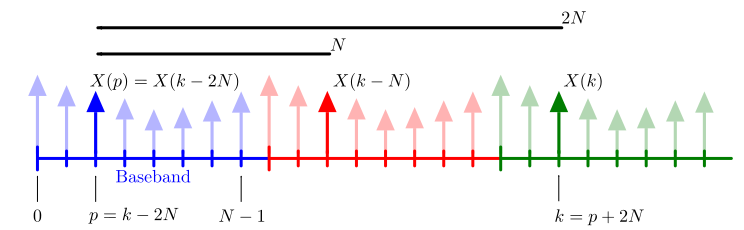
\includegraphics[width=\textwidth]{baseband.pdf}
\par\end{centering}
\caption{Illustration of the baseband and higher bands.}
\label{fig:baseband}
\end{figure*}


\levelstay{DFT of a baseband complex exponential}

The DFT of an exponential is of fundamental importance.
Given a signal $x(n)=\exp(i2\pi nq/N)$ with $q$ in the baseband, the DFT value at a frequency $k$ in the baseband is
\begin{align}
  X(k) =& \sum_{n=0}^{N-1} e^{i2\pi nq/N}e^{-i2\pi nk/N} \\
  =& N \delta_{k, q} \, .
\end{align}
Of course, as already discussed, the DFT value for $k$'s outside the baseband are uniquely determined by those in the baseband.
In particular, in this case we have
\begin{equation}
  X(k + mN) = N \delta_{k, q} \, .
\end{equation}
This is a series of delta peaks separated from each other by $N$ units in frequency space.
Note that this agrees with our previous discussion which said that all DFT coefficients separated by $N$ must be equal.
As previously explained, it makes sense to ignore the coefficients for $k$ outside the baseband, in which case the DFT of the exponential becomes
\begin{equation}
X(k) = \delta_{k,p} \label{eq:dftExponential}
\end{equation}
where $p$ is the \emph{unique} integer in the baseband which is related to $q$ by translation by an integer multiple of $N$, ie. $p=q-mN$.

\levelstay{Aliasing}

What happens if we have an exponential signal $x(n)=e^{i2\pi nq/N}$ when $q$ is outside the baseband?
According to (\ref{eq:dftExponential}) we get a delta peak $\delta_{k,p}$ with $p$ in the baseband and $p = q-mN$ for some integer $m$.
The value of $m$ doesn't matter, the point is that an exponential at a frequency $q$ outside the baseband has the same DFT as an exponential with Fourier frequency $p$ inside the baseband.
A consequence is that if you measure a signal $A\exp\left[i2\pi nq/N\right]+B\exp\left[i2\pi n(q+mN)/N\right]$ the DFT will look exactly the same as if you had measured $(A+B)\exp\left[i2\pi nq/N\right]$.
The indistinguishability of these signals is called $\textbf{aliasing}$, because the actual signal at higher frequency $q+mN$ \emph{looks} like the lower frequency $q$ in frequency space.
What's going on here is that signals with Fourier frequency outside the baseband oscillate more than once per data point, but since we only sample once per data point these oscillations are hidden and the DFT sees the signal at a lower frequency.

In calculations it can be annoying to replace $q$ values outside the baseband by $p+mN$ explicitly.
Instead, you can just do the replacement once the computation is complete.
To get this right use the following \textbf{rules for computing DFTs}
\begin{equation}
  \left[ \textrm{DFT}\left( e^{i2\pi nq/N} \right)\right](k) = \delta_{k,q} \, .
\end{equation}
Then, if $q$ is outside the baseband, at the end of the calculation find the corresponding $p$ inside the baseband and make the replacement
\begin{equation}
  \delta_{k,q} \rightarrow \delta_{k,p} \quad q=p+mN \, . \label{eq:aliasReplacement}
\end{equation}


\section{Appendix - Sums for Fourier Series power analysis}

The sum we want to compute is\begin{eqnarray*}
S & = & \frac{1}{4}\sum_{k}\left[\textrm{sinc}(\xi-k)+\textrm{sinc}(\xi+k)\right.\\
 & + & \left.2\cos(2\pi\xi)\textrm{sinc}(\xi-k)\textrm{sinc}(\xi+k)\right]\end{eqnarray*}
We write this as\[
S=\frac{1}{4}\left[S_{1}+S_{1}+2\cos(2\pi\xi)S_{2}\right]\]
The first sum we need to do is\[
S_{1}=\sum_{k=-\infty}^{\infty}\textrm{sinc}(\xi-k)^{2}\]
This is easy if we use the Poisson summation formula which states
that\[
\sum_{n}f(n-\xi)=\sum_{m}\tilde{f}(m)e^{-i2\pi\xi m}\]
Using this formula we get\begin{eqnarray*}
S_{1} & = & \sum_{m}\widetilde{\textrm{sinc}^{2}\left(m\right)}e^{-i2\pi\xi m}\\
S_{1} & = & \sum_{m}\textrm{tri}(m)e^{-i2\pi\xi m}\end{eqnarray*}
where $\textrm{tri}(x)$ is a triangle function; ie, $\textrm{tri}(x)=x+1$
for $-1<x<0$ and $\textrm{tri}(x)=-x+1$ for $0<x<1$, and $\textrm{tri}(x)=0$
elsewhere. Since $\textrm{tri}(m)$ is only nonzero for $m=0$ the
sum is simply\[
S_{1}=1\]
The second sum we need to do is\[
S_{2}=\sum_{k=-\infty}^{\infty}\textrm{sinc}(\xi-k)\textrm{sinc}(\xi+k)\]
For now we just write $f$ instead of $\textrm{sinc}$ to tidy up
notation. Since $\textrm{sinc}$ is an even function we can stick
a minus sign in the first function like so,\[
S_{2}=\sum_{k}f(k-\xi)f(k+\xi)\]
From here we just crank,\begin{eqnarray*}
S_{2} & = & \sum_{k}\int_{q}\int_{q'}\tilde{f}(q)e^{i2\pi q(k-\xi)}\tilde{f}(q')e^{i2\pi q'(k+\xi)}\\
S_{2} & = & \int_{q}\int_{q'}\tilde{f}(q)\tilde{f}(q')e^{-i2\pi\xi(q-q')}\sum_{k}e^{i2\pi k(q+q')}\\
S_{2} & = & \int_{q}\int_{q'}\tilde{f}(q)\tilde{f}(q')e^{-i2\pi\xi(q-q')}\sum_{n}\delta(n-q-q')\\
S_{2} & = & \sum_{n}\int_{q}\tilde{f}(q)\tilde{f}(n-q)e^{-i2\pi\xi(2q-n)}\\
S_{2} & = & \sum_{n}e^{i2\pi\xi n}\int_{q}\tilde{f}(q)\tilde{f}(n-q)e^{i2\pi q(-2\xi)}\end{eqnarray*}
Now we have to pay attention to what $\tilde{f}$ actually is. It
turns out that the Fourier transform of the sinc function is simply
a constant function from -1/2 to +1/2 with unit amplitude. This means
that $\tilde{f}(q)\tilde{f}(n-q)$ is only nonzero for $n=0$, in
which case it is equal to $\tilde{f}(q)$. Therefore we get\begin{eqnarray*}
S_{2} & = & \int_{q}\tilde{f}(q)e^{i2\pi q(-2\xi)}\\
S_{2} & = & f(-2\xi)\\
S_{2} & = & \textrm{sinc}(-2\xi)\\
S_{2} & = & \textrm{sinc}(2\xi)\end{eqnarray*}
Plugging into the original expression gives\begin{eqnarray*}
S & = & \frac{1}{4}\left[1+1+2\cos(2\pi\xi)\textrm{sinc}(2\xi)\right]\\
S & = & \frac{1}{2}\left[1+\cos(2\pi\xi)\textrm{sinc}(2\xi)\right]\\
S & = & \frac{1}{2}\left[1+\textrm{sinc}(4\xi)\right]\end{eqnarray*}
as stated in the main text.
